\chapter{Online survey}
This contains all the questions that were given to the participants of the online survey.
\begin{enumerate}
	\item What is your gender?
	\item What is your age?
	\item How many hours did you spend on video games last week?
	\begin{enumerate}
		\item 0 hours
		\item 1 to 3 hours
		\item 4 to 6 hours
		\item 7 to 10 hours
		\item More than 10 hours
	\end{enumerate}
	\item Which system/OS have you used to play video games in the last month?
	\begin{enumerate}
		\item Windows/Microsoft
		\item Mac/Apple
		\item Linux
		\item Other
	\end{enumerate}
	\item How much do you monthly spend on video games?
	\begin{enumerate}
		\item €0 to €20
		\item €21 to €40
		\item €41 to €60
		\item €60+
	\end{enumerate}
	\item How important is the price on a Gaming PC/Laptop/System for you?
	\begin{enumerate}
		\item Super important
		\item Very important
		\item Important
		\item Somewhat important
		\item Not important
	\end{enumerate}
	\item What kind of network connection do you use for gaming?
	\begin{enumerate}
		\item Wired connection
		\item Wireless connection (great range with low data rate)
		\item Wireless connection (short range with high data rate)
		\item I don't know
	\end{enumerate}
	\item What type of video games do you play?
	\begin{enumerate}
		\item Singleplayer
		\item Online Co-op
		\item Online multiplayer
	\end{enumerate}
\item Are you familiar with cloud gaming?
\begin{enumerate}
	\item Super familiar
	\item Very familiar
	\item Moderately familiar
	\item Somewhat familiar
	\item Not familiar
\end{enumerate}
\item What services have you heard of that allows to game via cloud?
\begin{enumerate}
	\item I don't know any services
	\item Other
\end{enumerate}
	\item Most cloud gaming services require a strong internet connection to make use of their service, do you have a strong internet connection at home?
	\begin{enumerate}
		\item Yes
		\item No
		\item Other
	\end{enumerate}
	\item When you play an online game, do you often have issues with latency/lag?
	\begin{enumerate}
		\item Yes
		\item No
		\item Other
	\end{enumerate}
	\item In cloud gaming, you stream a game through a data center on certain hardware, instead on a local computer or console in your home. What are your thoughts on this?
	\begin{enumerate}
		\item I like it, it saves a lot of space and is easy to access.
		\item I don't like it, and I would rather have personal ownership of gaming hardware/console.
		\item Other
	\end{enumerate}
	\item With cloud gaming, you're not owner of your games, unless you are attached to a monthly subscription. What are your thoughts on this?
	\begin{enumerate}
		\item I like it, because it saves money on purchasing games.
		\item I don't like it, and would rather purchase them on an online account then being attached to a subscription.
		\item Other
	\end{enumerate}
	\item Most cloud gaming services offer a montly subscription from €10 to €60, the monthly subscription for cloud gaming is:
	\begin{enumerate}
		\item Too cheap
		\item Somewhat cheap
		\item Reasonable
		\item Somewhat expensive
		\item Too expensive
	\end{enumerate}
	\item How interested are you in cloud gaming?
	\begin{enumerate}
		\item Super interested
		\item Very interested
		\item Moderately interested
		\item Slightly interested
		\item Not interested
	\end{enumerate}
	\item Which of the following are reasons that you might join a subscription for cloud gaming?
	\begin{enumerate}
		\item It serves a need of mine that is not currently being met
		\item I purchases someting similar in the past but need to replace it
		\item I'm looking for an alternative in gaming
		\item I'm not interested in buying new hardware at the moment
		\item Hardware is at scarcity and want to play video games soon
		\item I don't need a reason, and I don't need it
		\item Other
	\end{enumerate}
	\item Do you think cloud gaming has a future in the video game industry?
	\begin{enumerate}
		\item Yes
		\item No
		\item I'm not sure
	\end{enumerate}
	\item Based on your answers above, how likely are you to give cloud gaming a try?
	\begin{enumerate}
		\item Super likely
		\item Very likely
		\item Somewhat likely
		\item Slightly
		\item Not likely
	\end{enumerate}
	
\end{enumerate}
\chapter{RStudio}
What we have used to create our plots.
\begin{figure}[H]
	\centering
	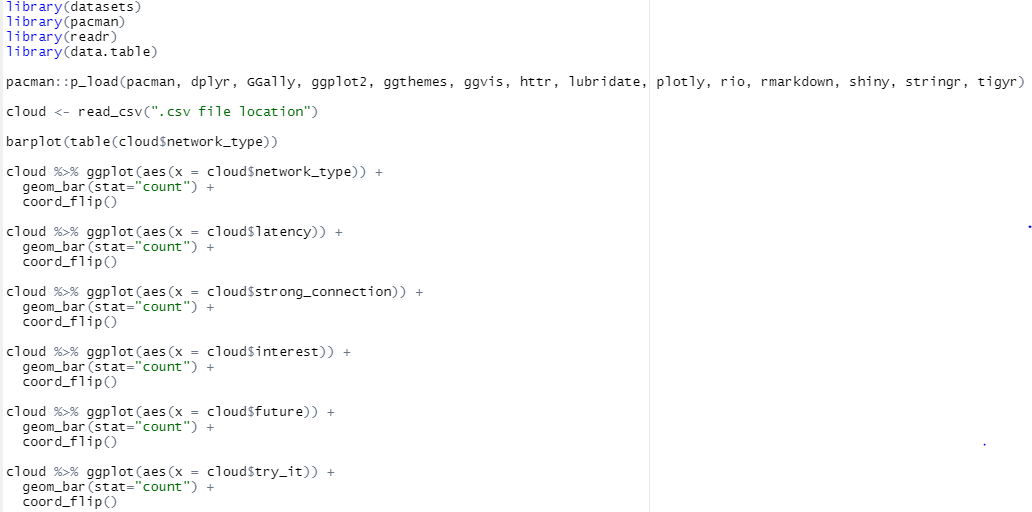
\includegraphics[width=16cm]{../img/R.png}
	\caption{Code for creating the necessary plots in R}
\end{figure}
